\documentclass[tikz,border=14pt]{standalone}
\usepackage{tikz}
\usepackage{amsmath}
\usetikzlibrary{arrows.meta,fit,backgrounds}

\definecolor{cGate} {RGB}{50, 100, 185}
\definecolor{cExp}  {RGB}{120, 45, 175}
\definecolor{cOut}  {RGB}{185, 45,  45}
\definecolor{cNote} {RGB}{80,  80,  80}

\tikzset{
  B/.style   = {draw, thick, rounded corners=4pt, text centered, font=\small,
                minimum height=10mm},
  tokB/.style  = {B, fill=gray!10,    draw=gray!55,  minimum width=30mm},
  gateB/.style = {B, fill=cGate!14,   draw=cGate!70, minimum width=36mm},
  expB/.style  = {B, fill=cExp!14,    draw=cExp!70,  minimum width=34mm,
                  minimum height=14mm},
  wgtB/.style  = {B, fill=cGate!8,    draw=cGate!45, minimum width=30mm},
  outB/.style  = {B, fill=cOut!14,    draw=cOut!75,  minimum width=30mm},
  sumB/.style  = {draw, circle, thick, fill=white, minimum size=9mm, font=\large},
  noteB/.style = {draw=cNote!40, rounded corners=4pt, fill=gray!5,
                  font=\scriptsize, text=cNote, inner sep=6pt, align=left},
  A/.style = {-Stealth, thick},
}

\begin{document}
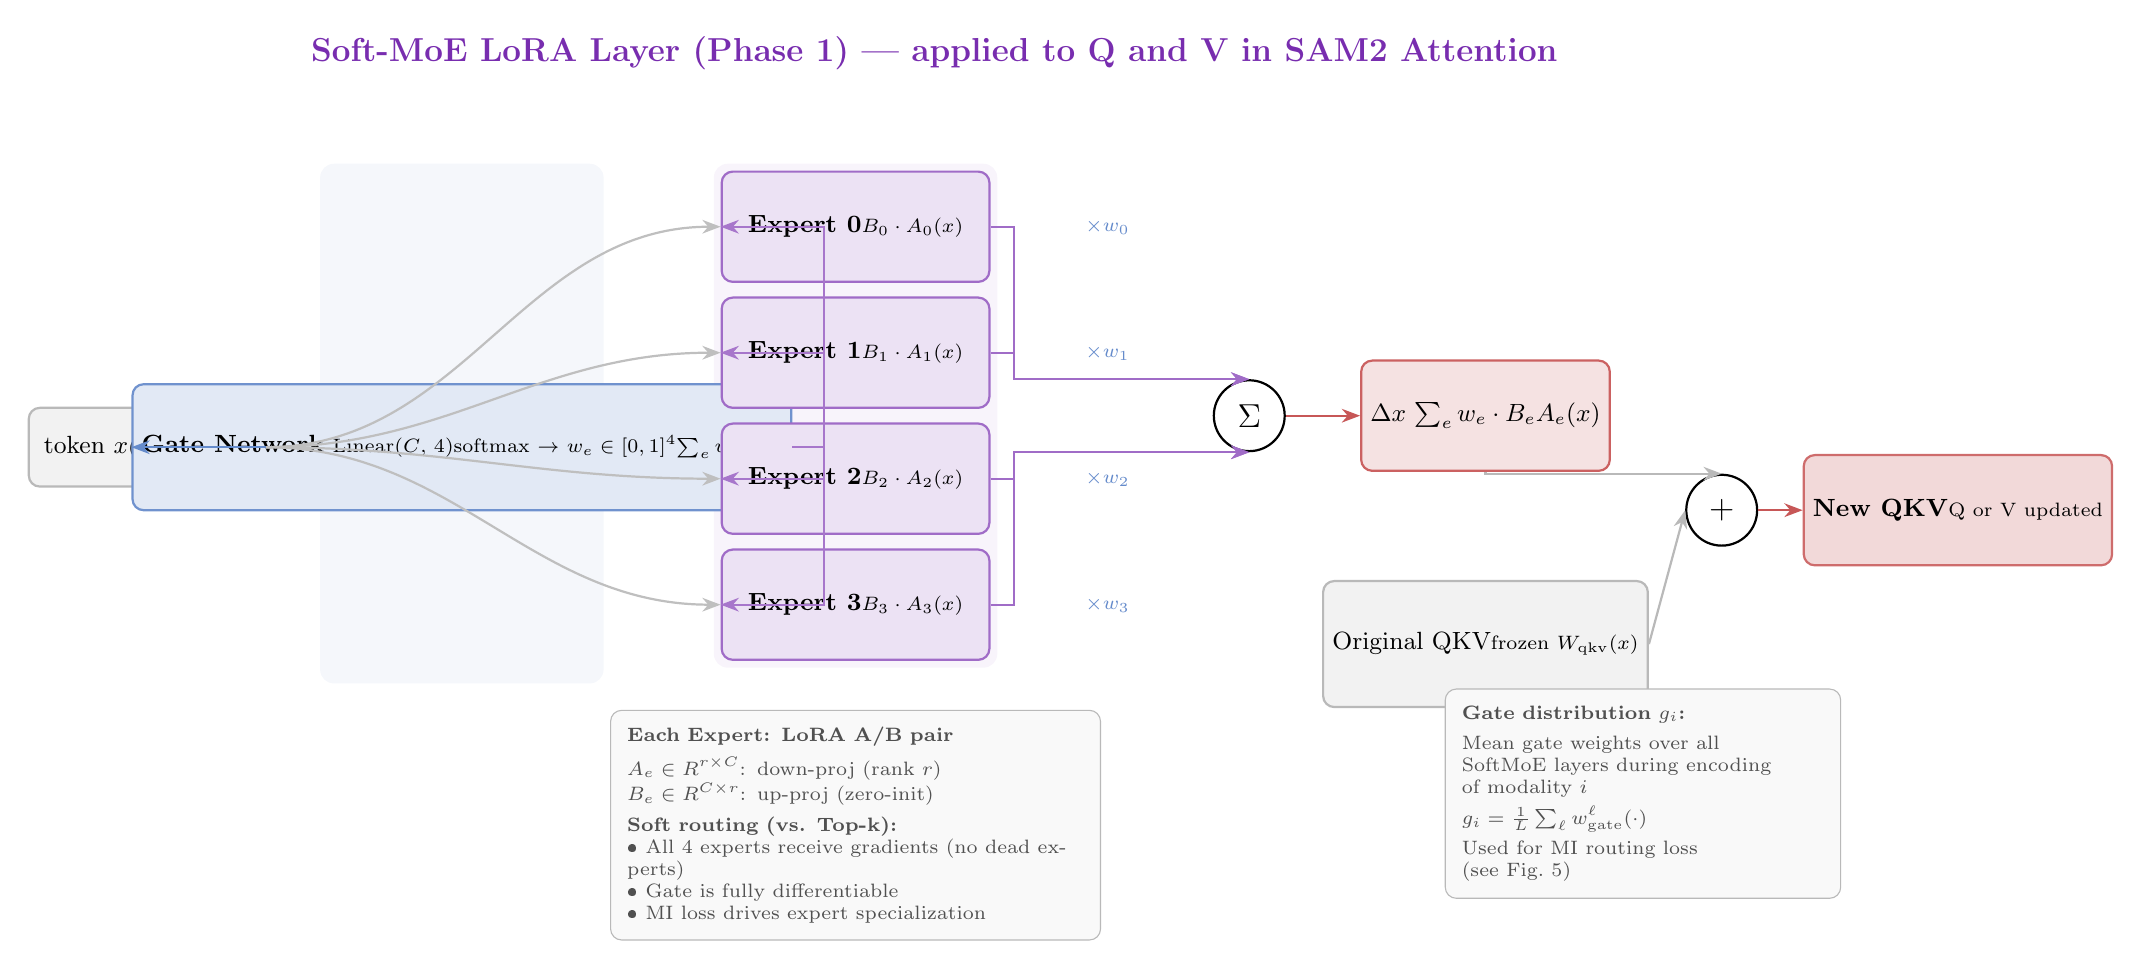
\begin{tikzpicture}

%% ─── Title ──────────────────────────────────────────────────────
\node[font=\large\bfseries, text=cExp] at (10.0, 4.0)
  {Soft-MoE LoRA Layer (Phase~1) --- applied to Q and V in SAM2 Attention};

%% ─── Input token ─────────────────────────────────────────────
\node[tokB] (x) at (0.0,-1.0) {token $x$\\{\scriptsize $(B,H,W,C)$}};

%% ─── Gate network ────────────────────────────────────────────
\node[gateB, minimum height=16mm] (gate) at (4.0,-1.0)
  {\textbf{Gate Network}\\[3pt]
   {\scriptsize Linear($C$, 4)}\\
   {\scriptsize softmax $\to$ $w_e \in [0,1]^4$}\\
   {\scriptsize $\sum_e w_e = 1$}};

\draw[A, cGate!75] (x.east)--(gate.west);

%% ─── 4 Experts ───────────────────────────────────────────────
\node[expB] (e0) at (9.0,  1.8)
  {\textbf{Expert 0}\\{\scriptsize $B_0 \cdot A_0(x)$}};
\node[expB] (e1) at (9.0,  0.2)
  {\textbf{Expert 1}\\{\scriptsize $B_1 \cdot A_1(x)$}};
\node[expB] (e2) at (9.0, -1.4)
  {\textbf{Expert 2}\\{\scriptsize $B_2 \cdot A_2(x)$}};
\node[expB] (e3) at (9.0, -3.0)
  {\textbf{Expert 3}\\{\scriptsize $B_3 \cdot A_3(x)$}};

%% arrows from gate to experts (and x to experts)
\draw[A, cExp!65] (gate.east)--++(4mm,0) |- (e0.west);
\draw[A, cExp!65] (gate.east)--++(4mm,0) |- (e1.west);
\draw[A, cExp!65] (gate.east)--++(4mm,0) |- (e2.west);
\draw[A, cExp!65] (gate.east)--++(4mm,0) |- (e3.west);

\draw[A, gray!50] (x.east) to[out=0,in=180] (e0.west);
\draw[A, gray!50] (x.east) to[out=0,in=180] (e1.west);
\draw[A, gray!50] (x.east) to[out=0,in=180] (e2.west);
\draw[A, gray!50] (x.east) to[out=0,in=180] (e3.west);

%% ─── Weighted sum ────────────────────────────────────────────
\node[sumB] (plus) at (14.0,-0.6) {$\Sigma$};

\draw[A, cExp!70] (e0.east)--++(3mm,0) |- (plus.north);
\draw[A, cExp!70] (e1.east)--++(3mm,0) |- (plus.north);
\draw[A, cExp!70] (e2.east)--++(3mm,0) |- (plus.south);
\draw[A, cExp!70] (e3.east)--++(3mm,0) |- (plus.south);

%% ─── Weight labels ───────────────────────────────────────────
\node[font=\scriptsize, text=cGate!75] at (12.2,  1.8) {$\times w_0$};
\node[font=\scriptsize, text=cGate!75] at (12.2,  0.2) {$\times w_1$};
\node[font=\scriptsize, text=cGate!75] at (12.2, -1.4) {$\times w_2$};
\node[font=\scriptsize, text=cGate!75] at (12.2, -3.0) {$\times w_3$};

%% ─── LoRA delta output ───────────────────────────────────────
\node[outB, minimum height=14mm] (delta) at (17.0,-0.6)
  {\textbf{$\Delta x$}\\[3pt]
   {\small $\sum_e w_e\cdot B_e A_e(x)$}};

\draw[A, cOut!80, thick] (plus.east)--(delta.west);

%% ─── Added to original QKV ──────────────────────────────────
\node[tokB, minimum height=16mm] (qkv) at (17.0,-3.5)
  {Original QKV\\{\scriptsize frozen $W_\text{qkv}(x)$}};

\node[sumB] (add) at (20.0,-1.8) {$+$};

\draw[A, gray!55] (delta.south)--(delta.south |- add.north)--(add.north);
\draw[A, gray!55] (qkv.east)  -- (add.west);

\node[B, fill=cOut!18, draw=cOut!70, minimum width=28mm,
      minimum height=14mm] (out) at (23.0,-1.8)
  {\textbf{New QKV}\\{\scriptsize Q or V updated}};
\draw[A, cOut!80, thick] (add.east)--(out.west);

%% ─── Expert structure note ───────────────────────────────────
\node[noteB, text width=58mm] at (9.0,-5.8)
  {\textbf{Each Expert: LoRA A/B pair}\\[3pt]
   $A_e \in \mathbb{R}^{r \times C}$: down-proj (rank $r$)\\
   $B_e \in \mathbb{R}^{C \times r}$: up-proj (zero-init)\\[3pt]
   \textbf{Soft routing (vs. Top-k):}\\
   \textbullet~All 4 experts receive gradients (no dead experts)\\
   \textbullet~Gate is fully differentiable\\
   \textbullet~MI loss drives expert specialization};

%% ─── Gate distribution annotation ───────────────────────────
\node[noteB, text width=46mm] at (19.0,-5.4)
  {\textbf{Gate distribution $g_i$:}\\[3pt]
   Mean gate weights over all\\
   SoftMoE layers during encoding\\
   of modality $i$\\[3pt]
   $g_i = \frac{1}{L}\sum_\ell w^\ell_\text{gate}(\cdot)$\\[3pt]
   Used for MI routing loss\\ (see Fig.~5)};

%% ─── Column backgrounds ──────────────────────────────────────
\begin{scope}[on background layer]
  \fill[cGate!5, rounded corners=5pt]
    (2.2, 2.6) rectangle (5.8,-4.0);
  \fill[cExp!5, rounded corners=5pt]
    (7.2, 2.6) rectangle (10.8,-3.8);
\end{scope}

\end{tikzpicture}
\end{document}
